\subsection{Introducción}

En el presente trabajo de laboratorio se realizaron distintas mediciones utilizando el analizador de espectros. En primer lugar se compararó la distorsión armónica presente en distintos generadores de funciones; se procedió al análisis del espectro de algunas formas de ondas conocidas, como la cuadrada con duty cycle de $50\%$, la triangular y el tren de pulsos; posteriormente se modularon señales en AM y en FM y se observaron los espectros resultantes; por último se analizó el espectro de un sinc y un tren de deltas.

\subsection{Medición de distorsión armónica}
Como primera experiencia se midió la distorsión armónica (THD) de distintos generadores de funciones disponibles en el laboratorio. Para esto se generó una señal senoidal de $1$ Mhz y $350$ mVpp de amplitud, con el OUT TERM en HiZ; como la impedancia del analizador de espectros es de $50 \Omega$, la señal que llegó al analizador fue de aproximadamente $175$ mVpp ya que la mitad de la tensión cae sobre la impedancia del generador utilizado de $50 \Omega$. Una vez realizadas las mediciones, se compararon los valores de THD obtenidos con los recuperados de las hojas de datos de los fabricantes. Para el cálculo, se tomó la definición de THD como:
\begin{equation}
    THD=\frac{P_1+P_2+...+P_i}{P_0}
    \label{eq:THD}
\end{equation}
donde $P_0$ representa la potencia del armónico fundamental, y $P_i$ la potencia del i-ésimo armónico.

\begin{table}[H]
\centering
\begin{tabular}{@{}ccccccc@{}}
\toprule
\textbf{Generador} & $P_0$ & $P_1$ & $P_2$ & $P_3$ & $P_4$ & $P_5$ \\ \midrule
Picotest & -10dBm & -65dBm & -85dBm & NOAPR & NOAPR & NOAPR \\
Agilent & -11.4dBm & -55dBm & NOAPR & NOAPR & NOAPR & NOAPR \\
GW & -12.4dBm & -30dBm & -40dBm & -51dBm & -58dBm & -60dBm \\ \bottomrule
\end{tabular}
\caption{Tabla de mediciones realizadas. NOAPR significa potencia no apreciable o por debajo del piso de ruido del analizador de espectros.}
\end{table}

Luego de medir todas las potencias de los fundamentales y armónicos de los generadores $Agilent 3320a$, $Picotest G5100a$ y $GWGFG G8019G$ se calcularon las distorsiones armónicas de cada uno, resultando:

\begin{figure}[H]
\begin{subfigure}{0.33\textwidth}
\begin{table}[H]
\centering
\begin{tabular}{@{}cc@{}}
\toprule
Picotest & THD\\ \midrule
Datasheet & $\leq 0.06\%$  \\
Medido & $0.000319\%$ \\ \bottomrule
\end{tabular}
\caption{Mediciones del THD del picotest.}
\end{table}
\end{subfigure}
\begin{subfigure}{0.33\textwidth}
\begin{table}[H]
\centering
\begin{tabular}{@{}cc@{}}
\toprule
Agilent & THD \\ \midrule
Datasheet & $\leq 0.04\%$ \\
Medido & $0.0044\%$ \\ \bottomrule
\end{tabular}
\caption{Mediciones del THD del agilent.}
\end{table}
\end{subfigure}
\begin{subfigure}{0.33\textwidth}
\begin{table}[H]
\centering
\begin{tabular}{@{}cc@{}}
\toprule
Agilent & THD \\ \midrule
Datasheet & $-$ \\
Medido & $0.0044\%$ \\ \bottomrule
\end{tabular}
\caption{Mediciones del THD del GW.}
\end{table}
\end{subfigure}
\caption{Mediciones de la distorsión armónica total de los generadores. No se encontró hoja de datos para el generador GW.}
\end{figure}

A continuación se incluyen algunas imágenes de lo observado en el analizador de espectros. En las Figuras (\ref{fig:ag1}), (\ref{fig:ag2}) y (\ref{fig:ag3}) se presentan los picos para el generador Agilent; notamos que ya el segundo armónico es indistinguible. En las Figuras (\ref{fig:pico1}) se puede observar el espectro del generador Picotest, donde se aprecia que ya el segundo armónico tiene una amplitud muy Baja. No se puede observar un tercer armónico. Para el generador marca GW pudieron observarse más armónicos. En las Figuras (\ref{fig:gw0}) y (\ref{fig:gw1}) se observan el segundo y tercer armónico, respectivamente.

\begin{figure}[H]
  \centering
  \begin{minipage}[b]{0.4\textwidth}
    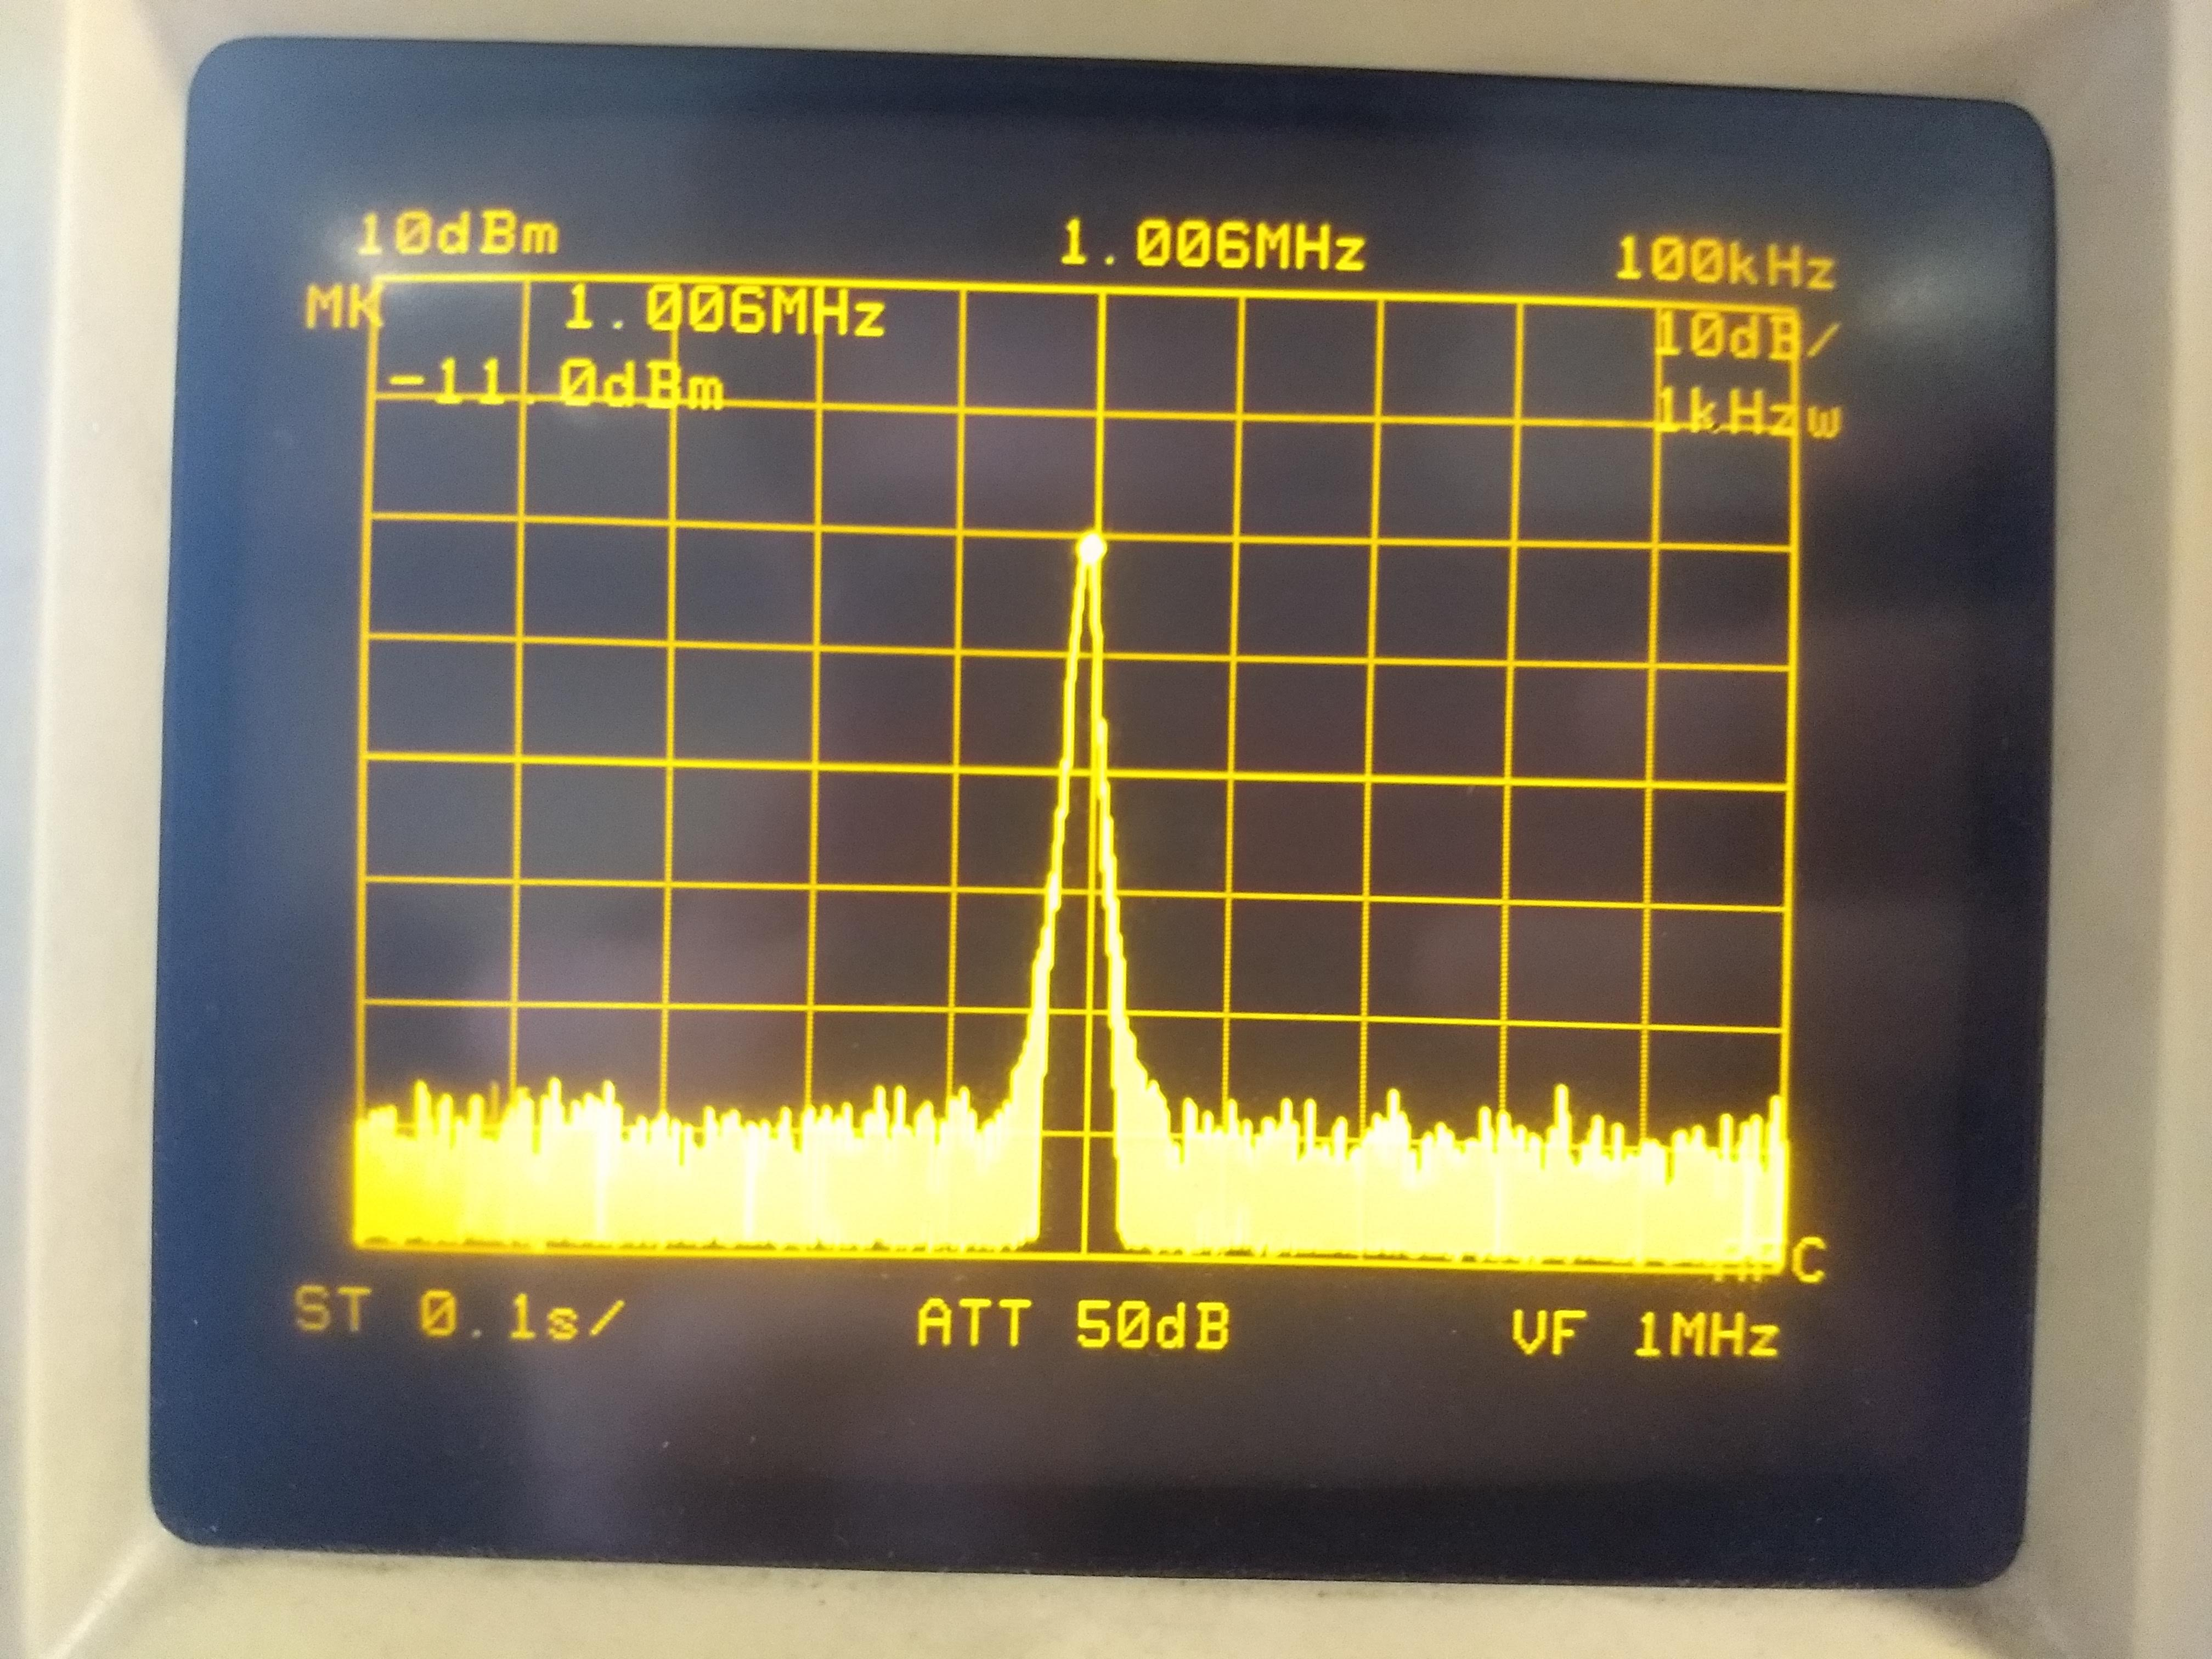
\includegraphics[width=\textwidth]{/ImagenesEjercicio1/agilentP0.jpg}
    \caption{Armónico fundamental para el generador Agilent}
    \label{fig:ag1}
  \end{minipage}
  \hfill
  \begin{minipage}[b]{0.4\textwidth}
    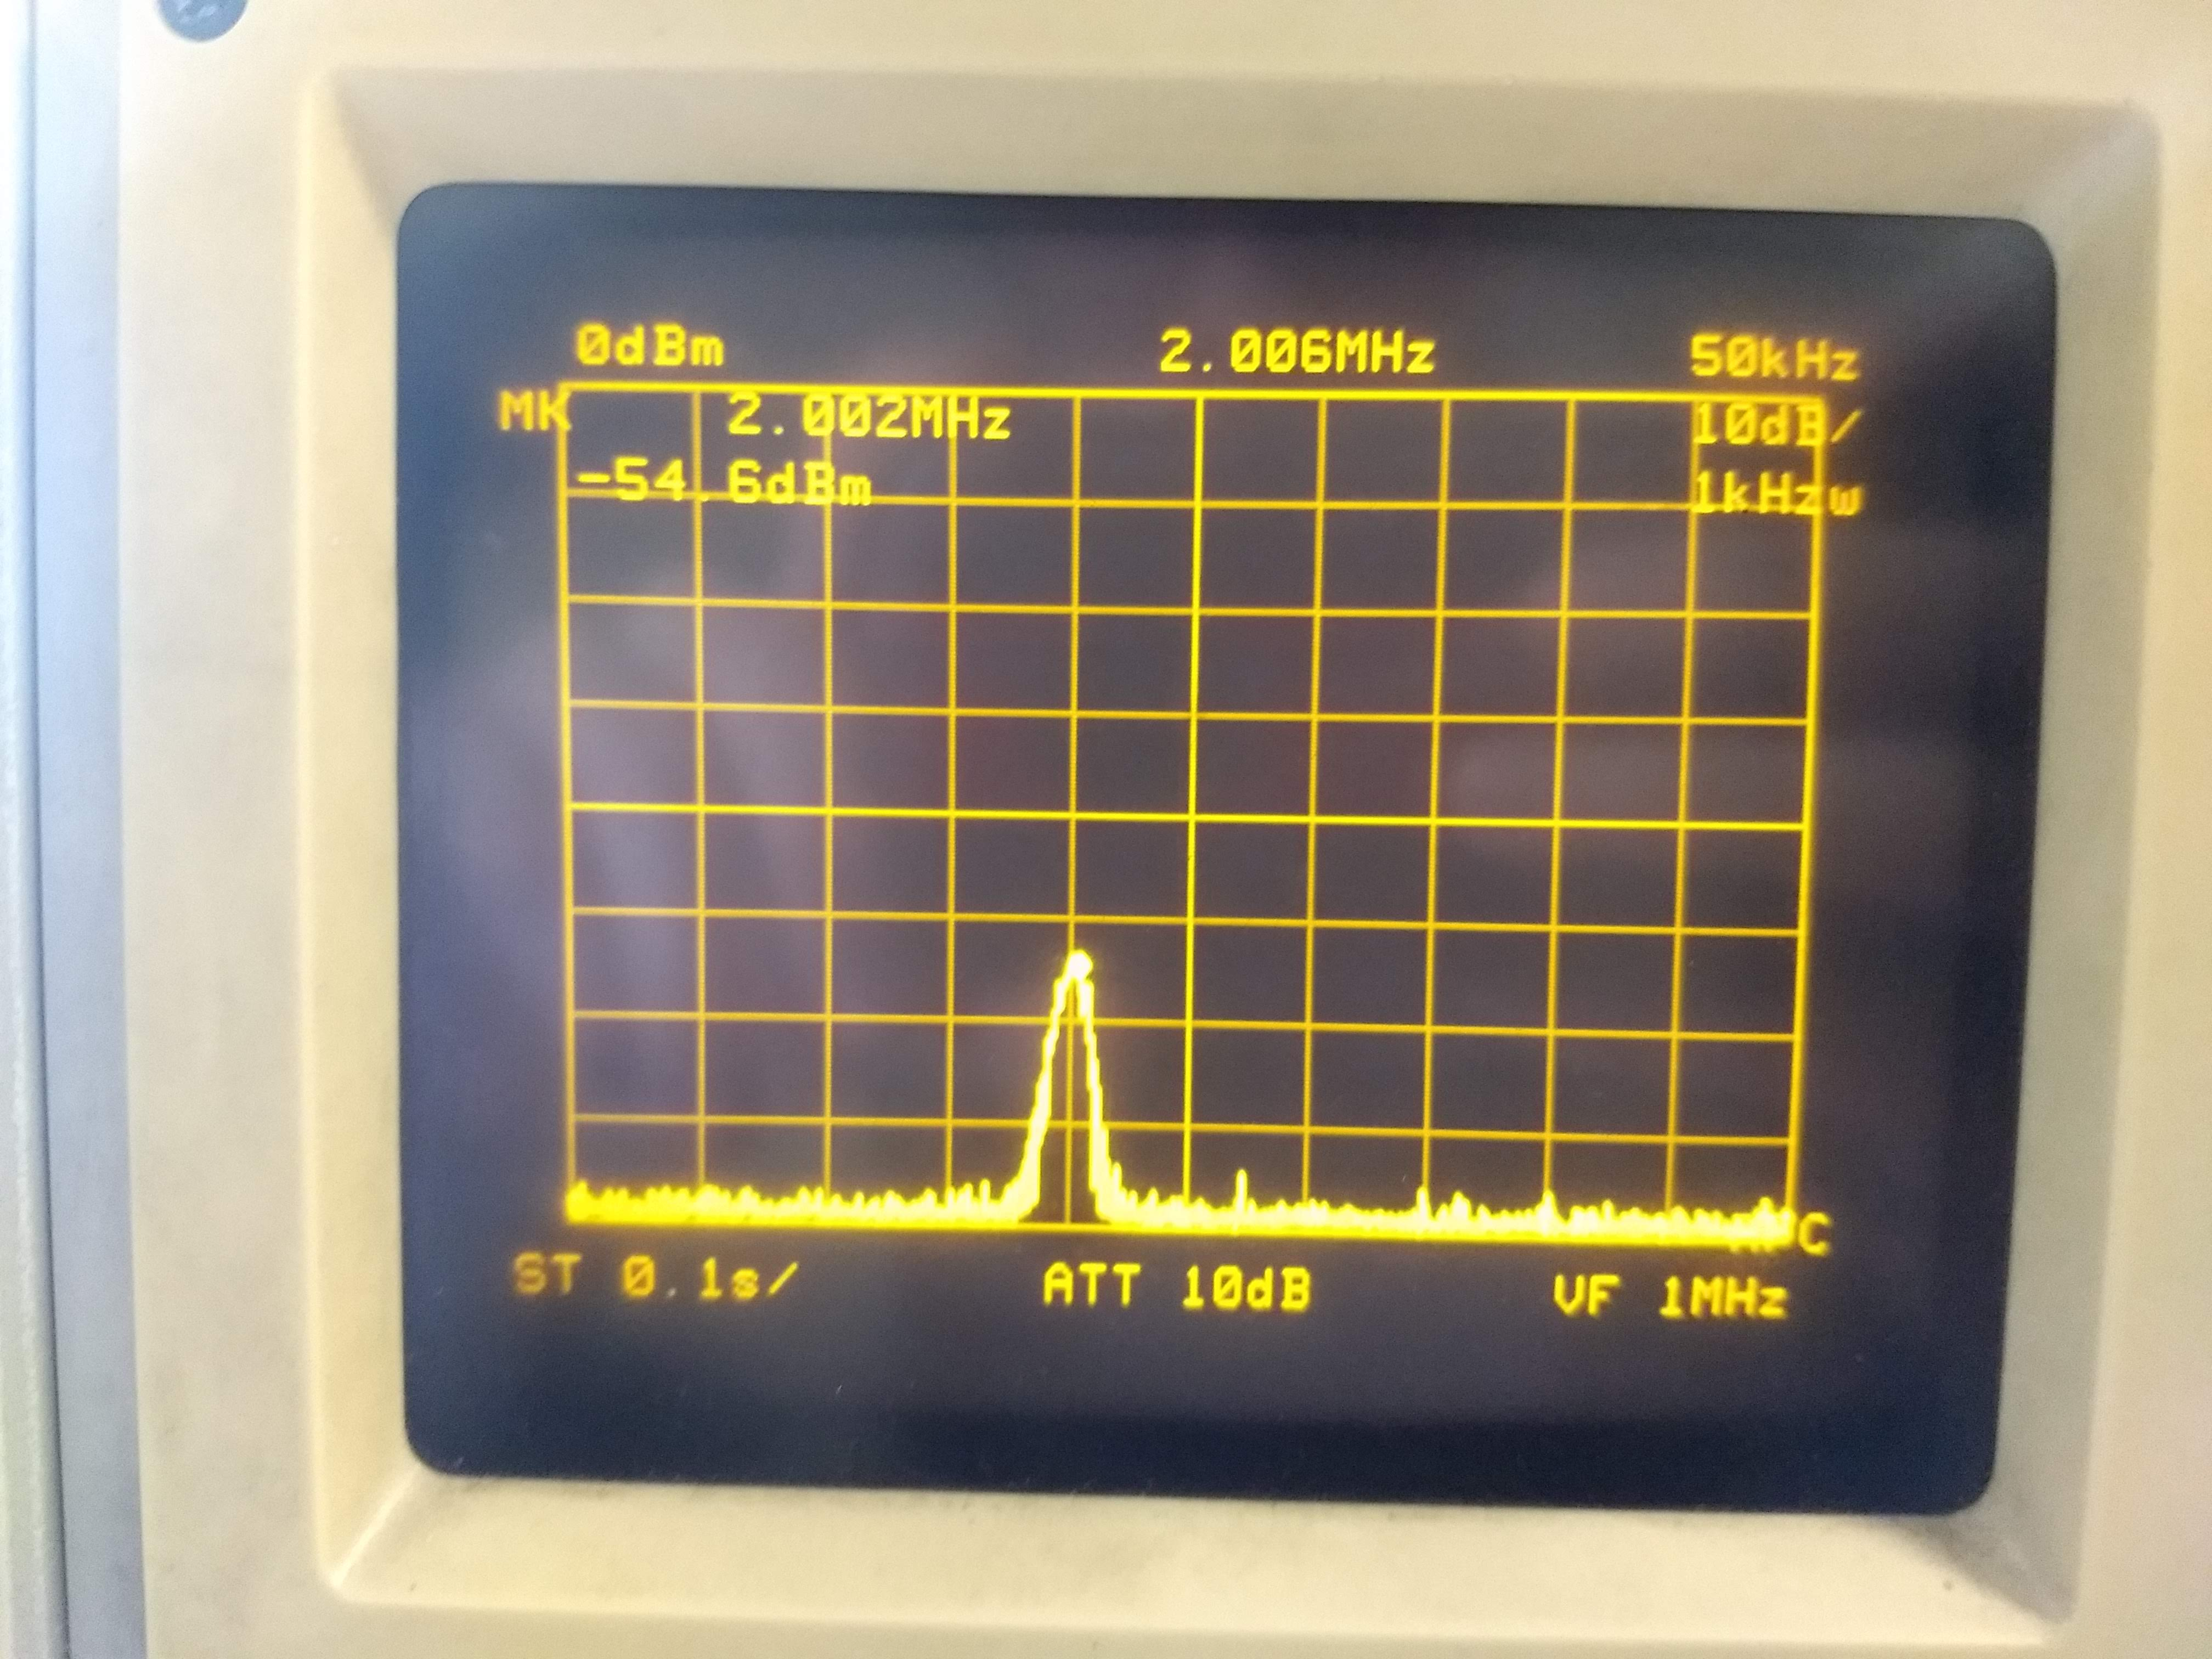
\includegraphics[width=\textwidth]{/ImagenesEjercicio1/agilentP1.jpg}
    \caption{Primer armónico para el generador Agilent}
    \label{fig:ag2}
  \end{minipage}
   \hfill
   \begin{minipage}[b]{0.4\textwidth}
    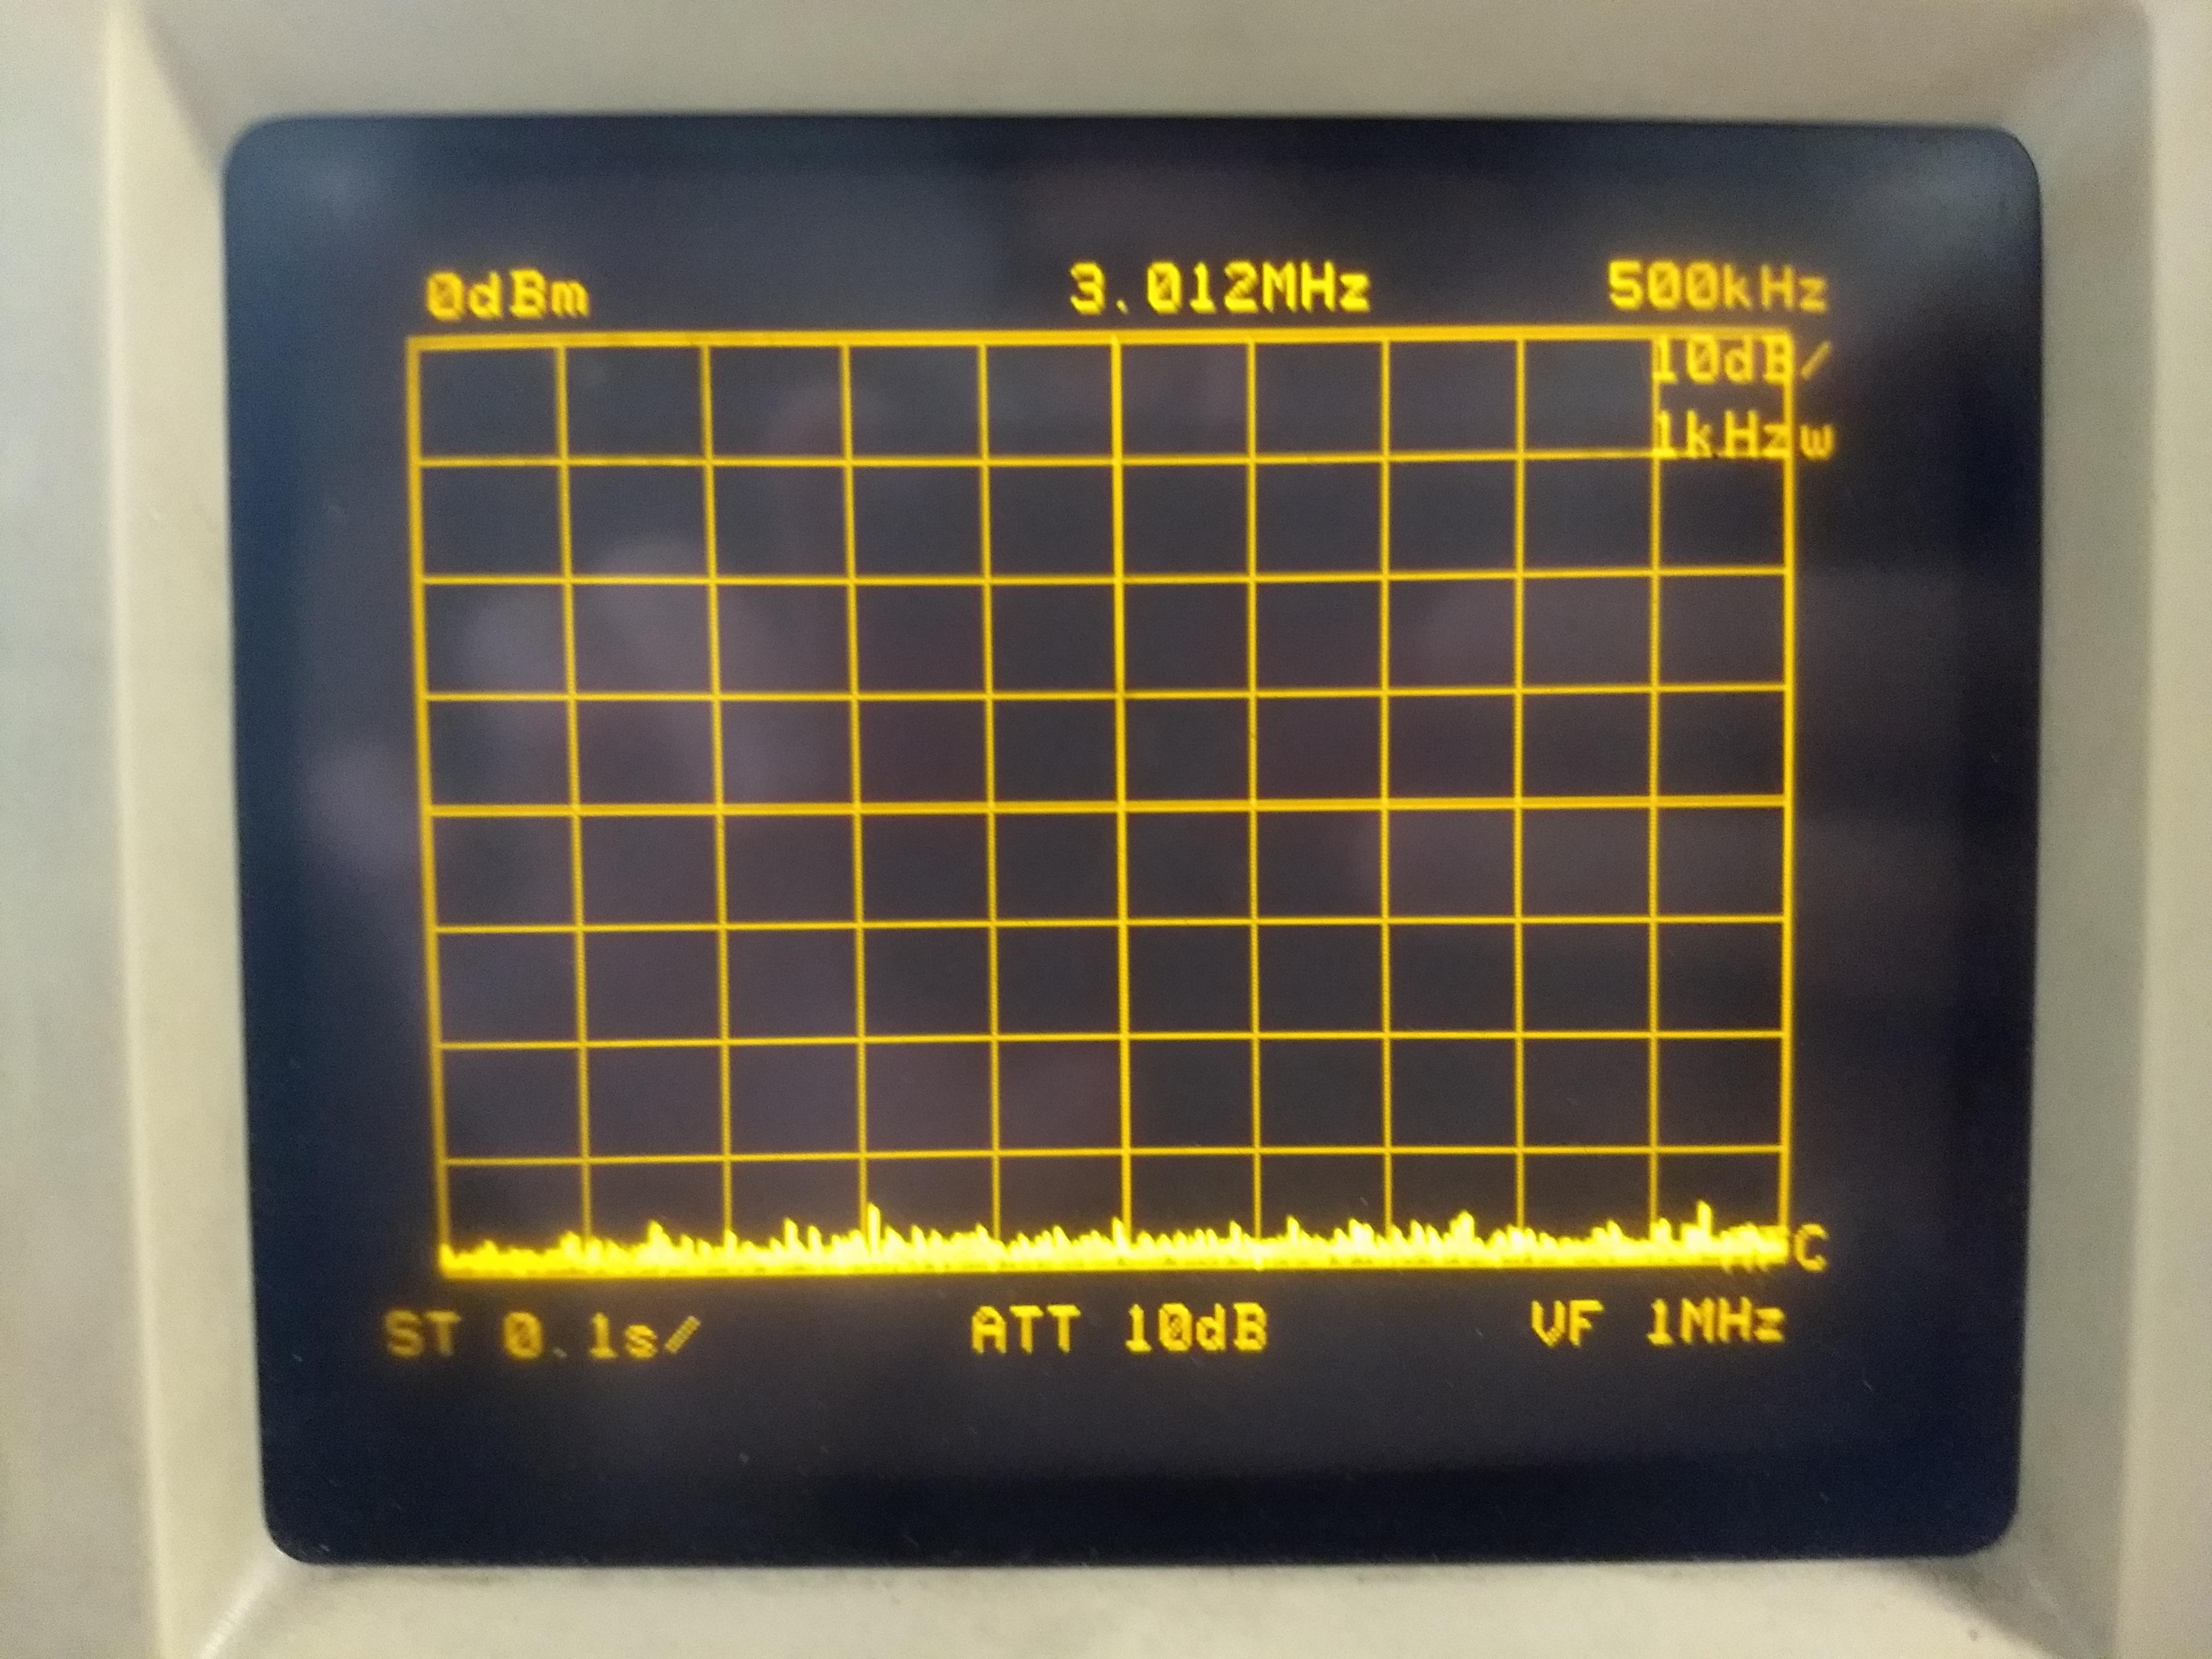
\includegraphics[width=\textwidth]{/ImagenesEjercicio1/agilentP2.jpg}
    \caption{Segundo armónico para el generador Agilent}
    \label{fig:ag3}
  \end{minipage}
\end{figure}

\begin{figure}[H]
	\centering
	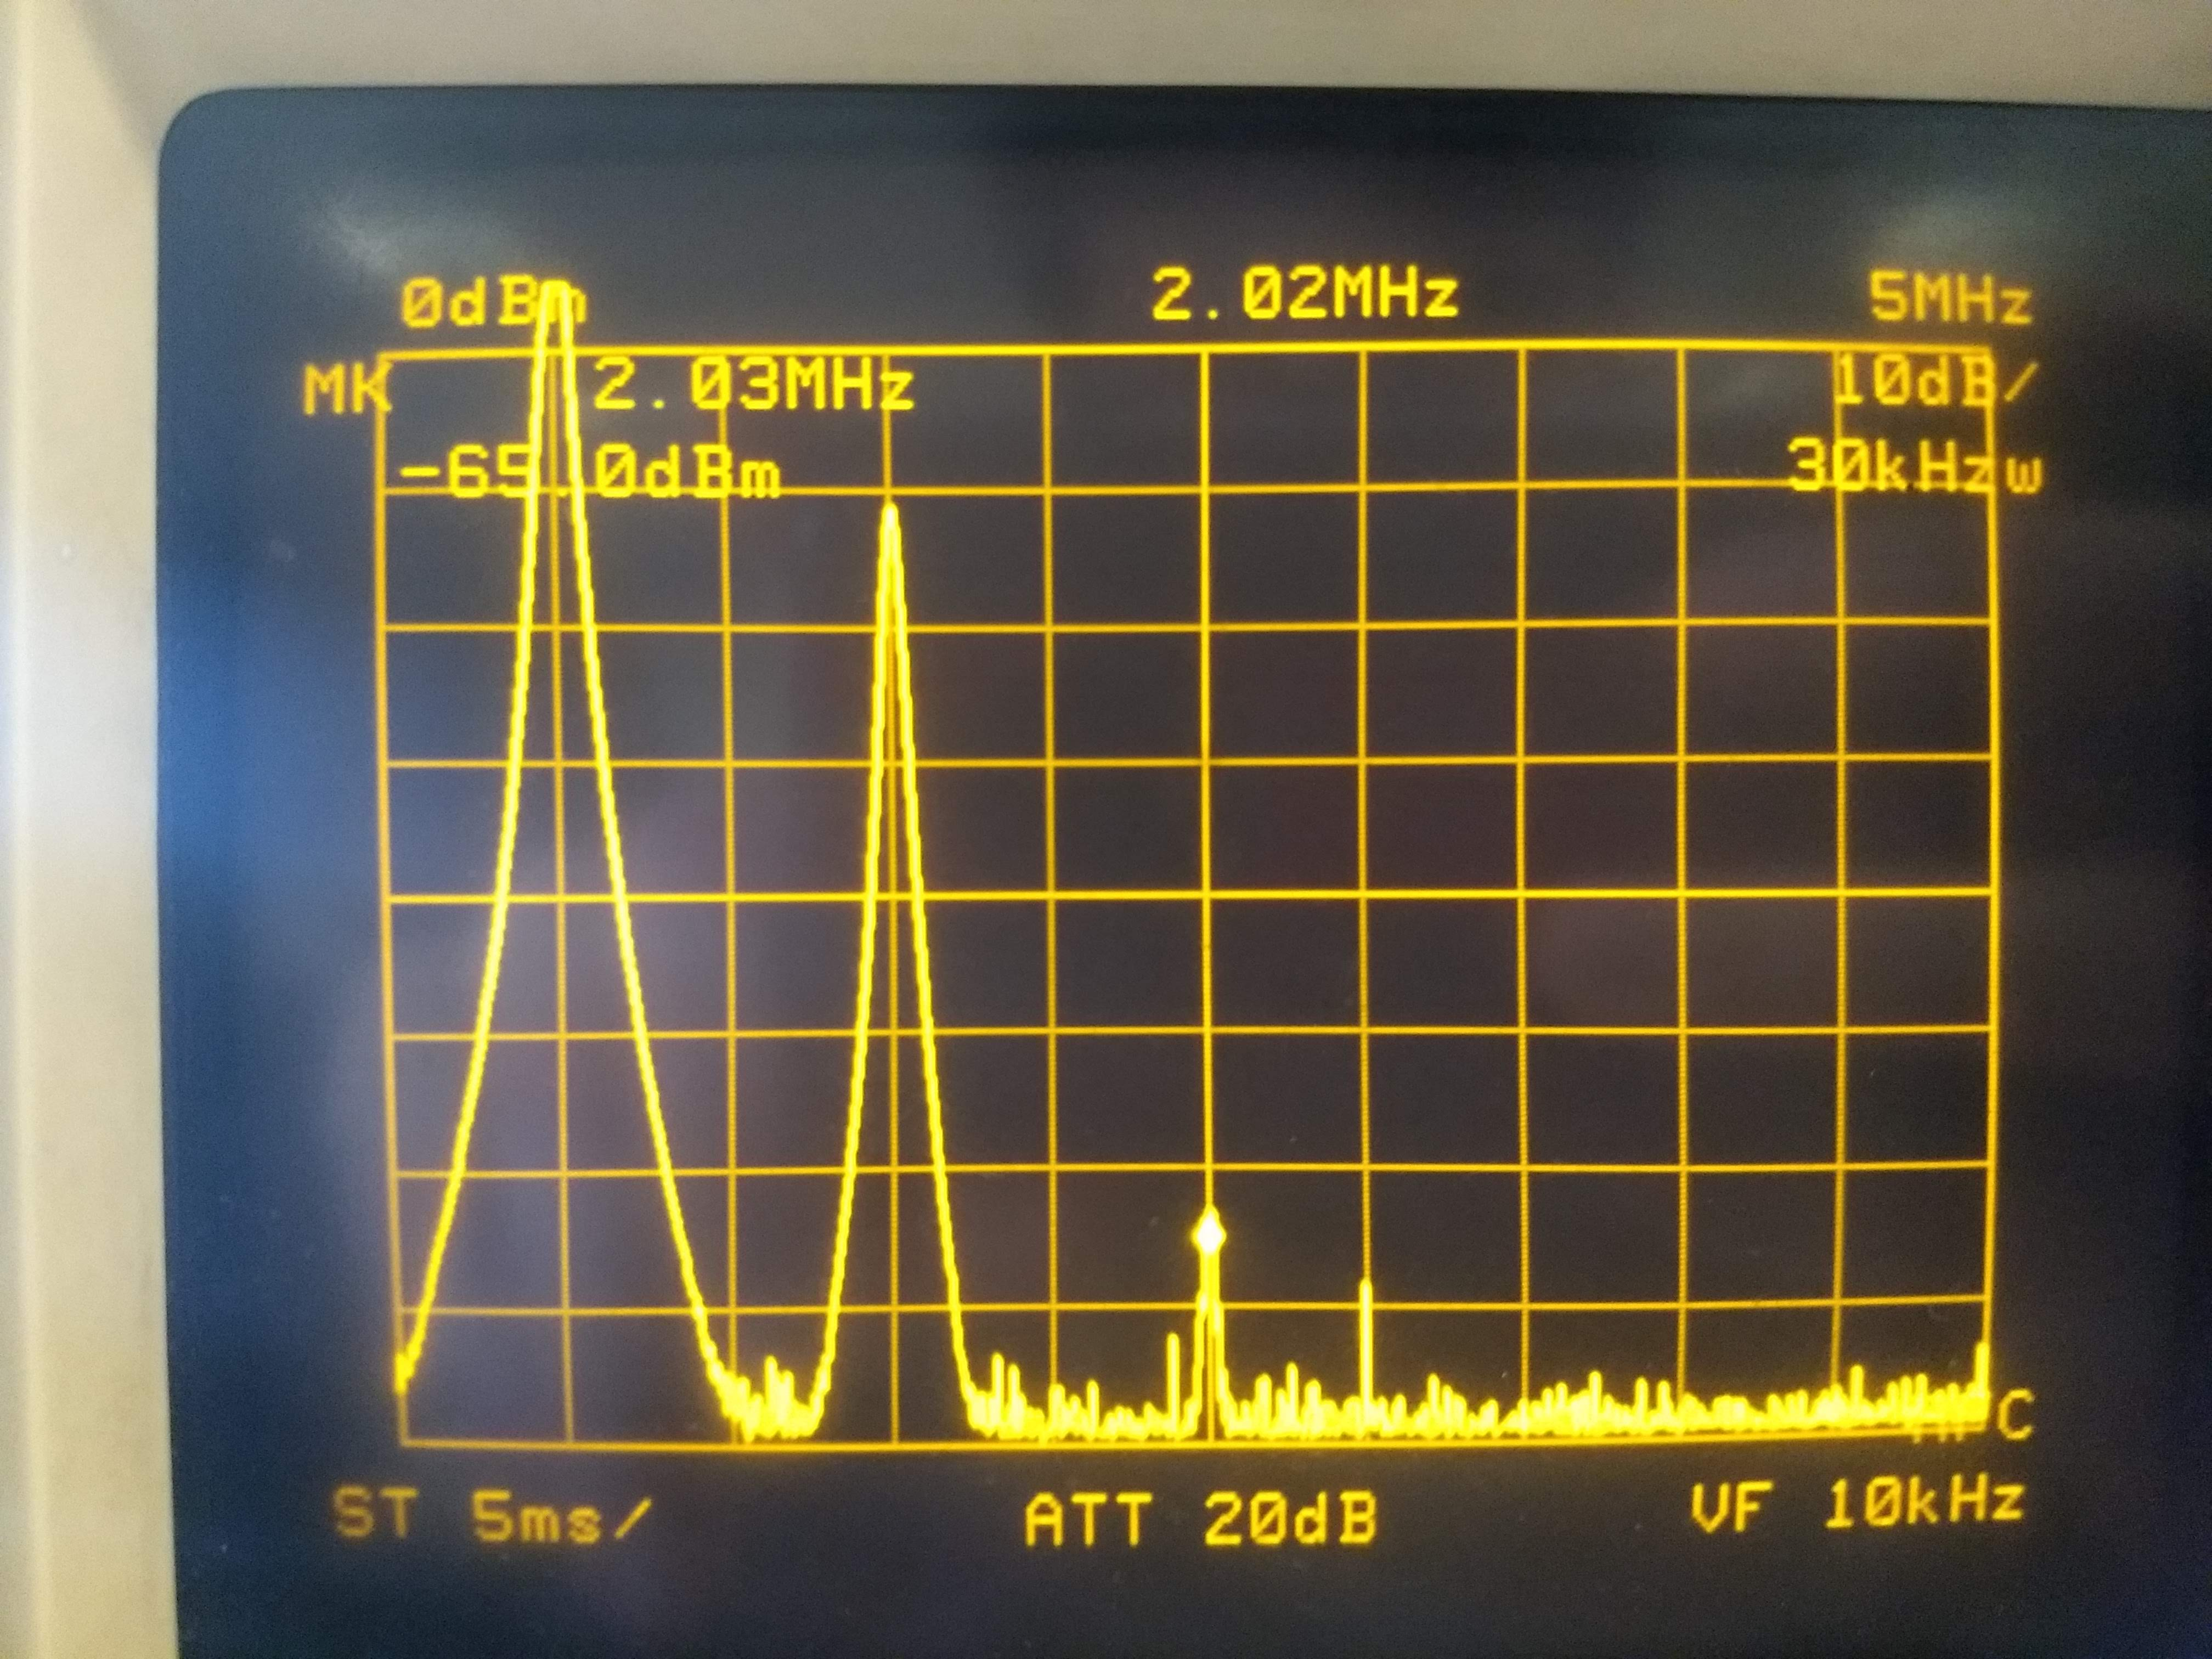
\includegraphics[width=0.7\textwidth]{/ImagenesEjercicio1/picotestP1.jpg}
\caption{Espectro para el generador Picotest}
	\label{fig:pico1}
\end{figure}

\begin{figure}[H]
  \centering
  \begin{minipage}[b]{0.4\textwidth}
    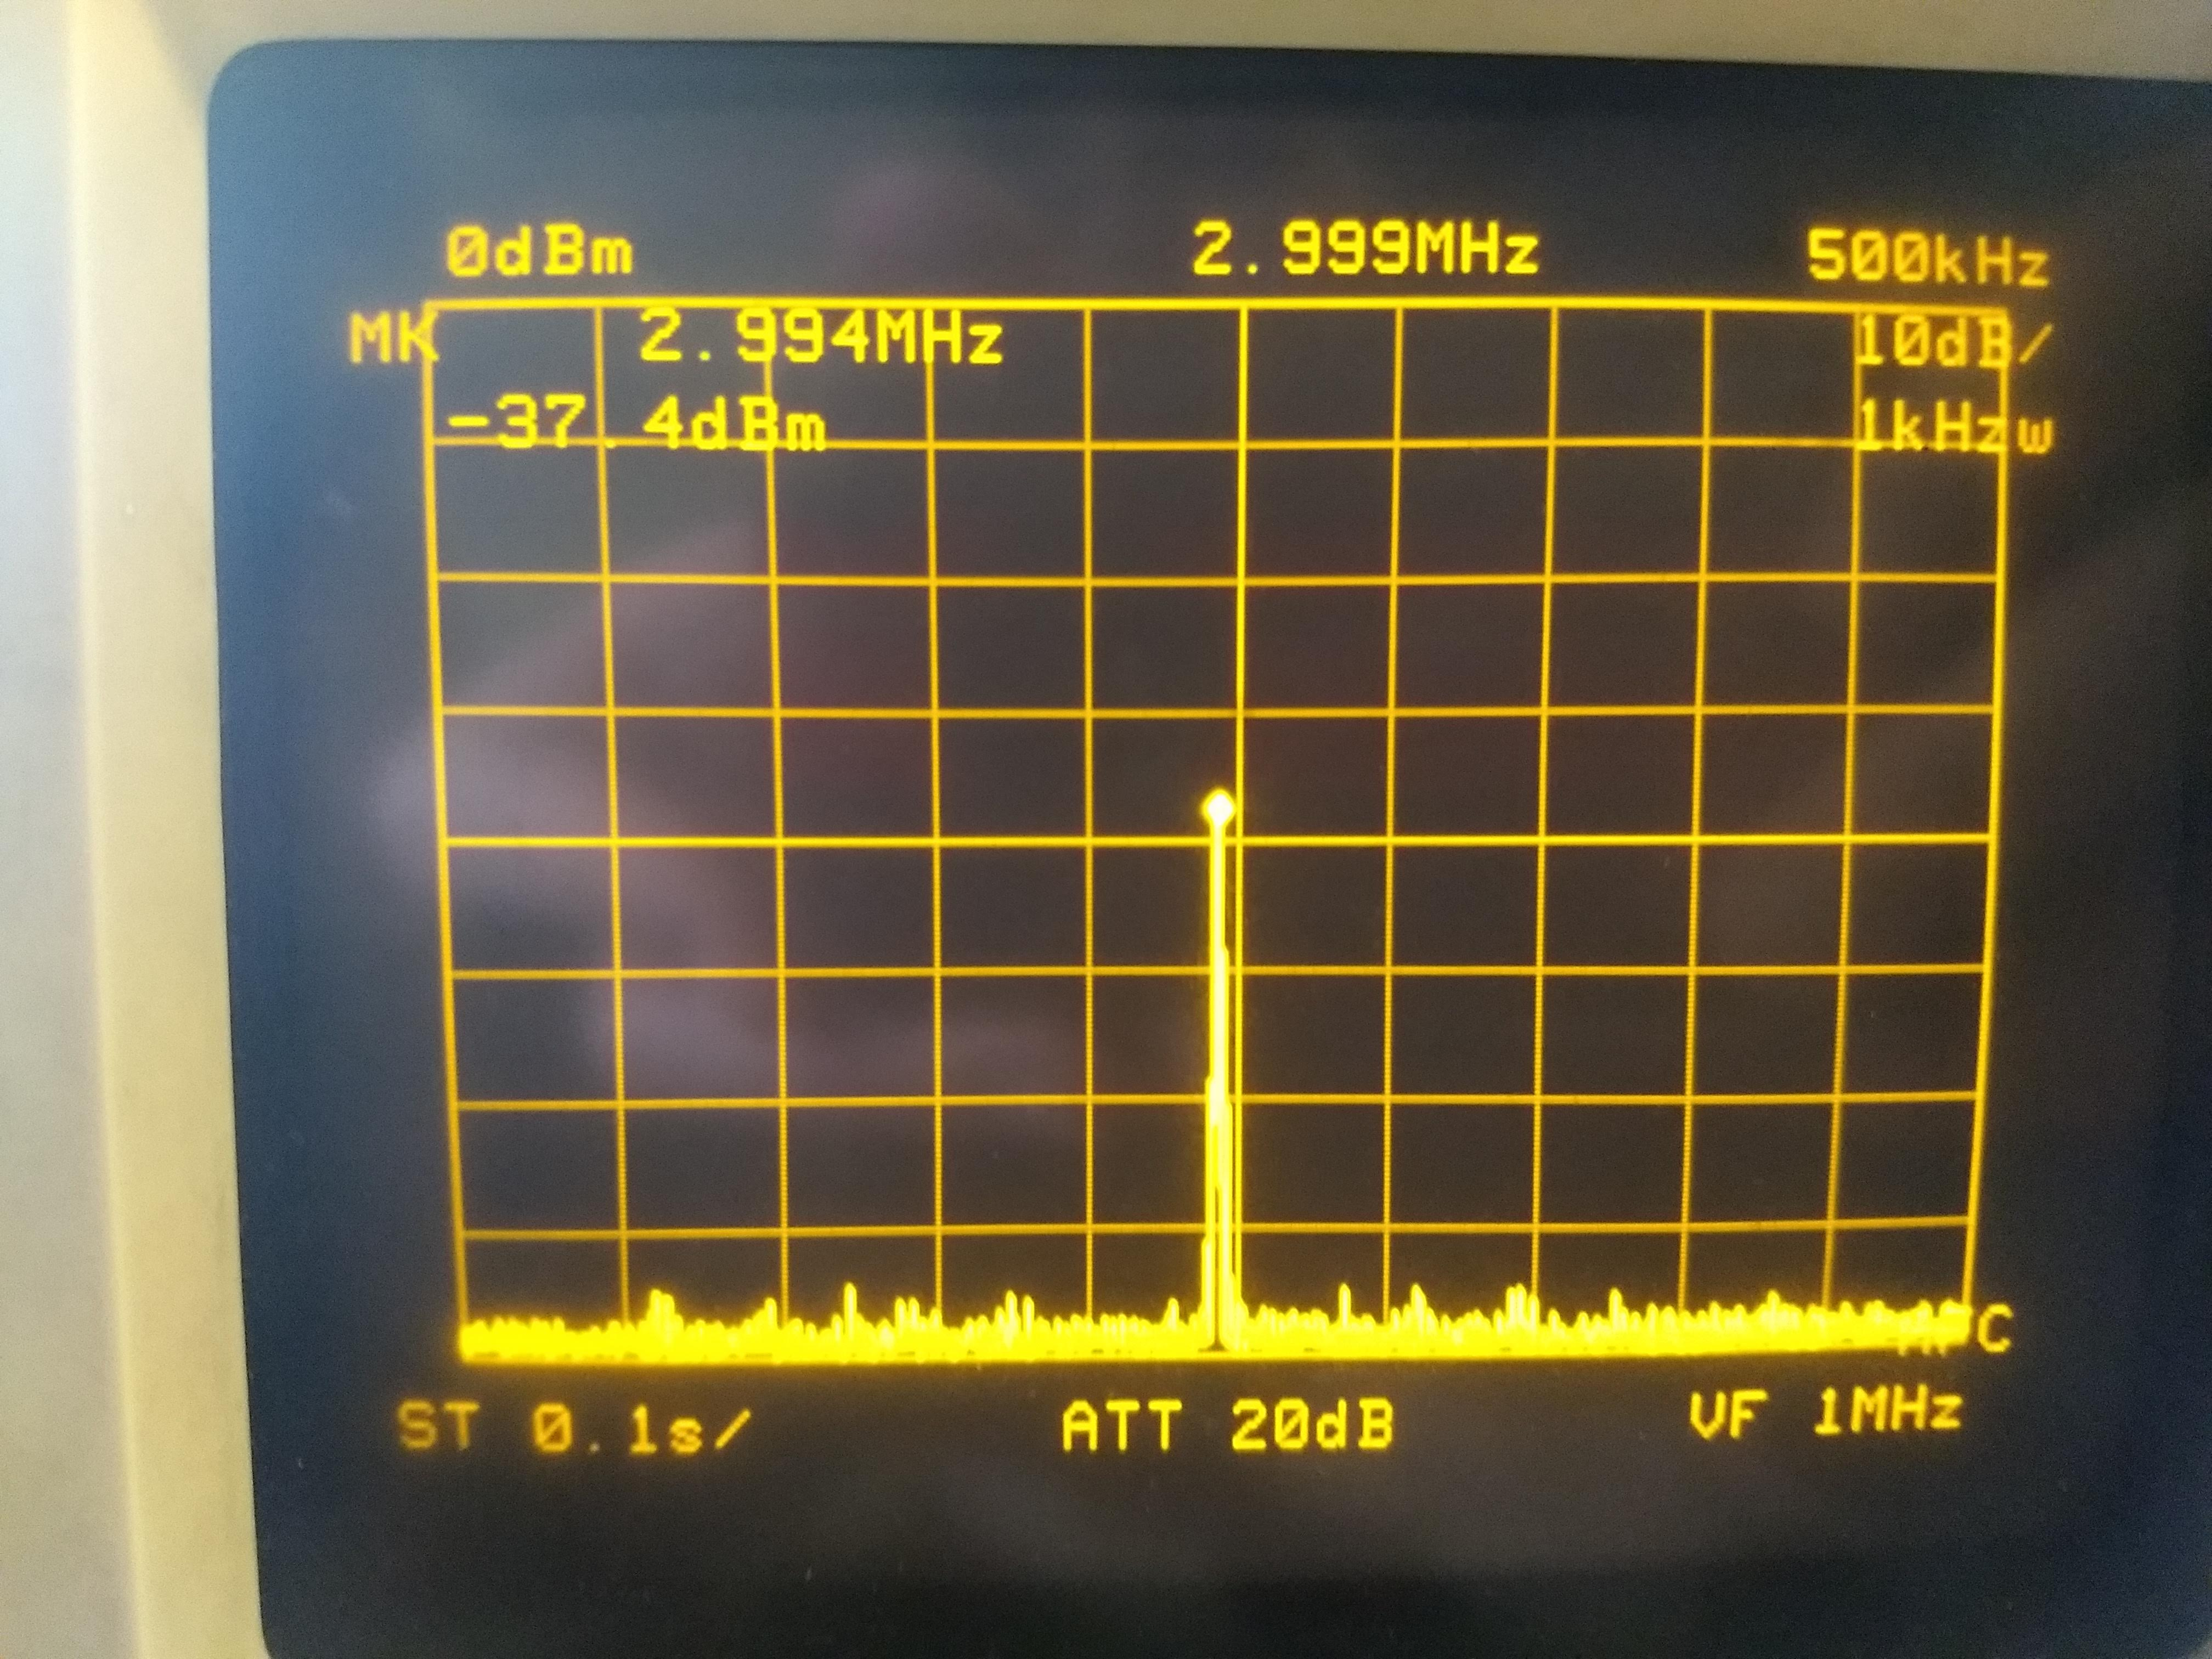
\includegraphics[width=\textwidth]{/ImagenesEjercicio1/gwP2.jpg}
    \caption{Segundo armónico para el generador GW}
    \label{fig:gw0}
  \end{minipage}
  \hfill
  \begin{minipage}[b]{0.4\textwidth}
    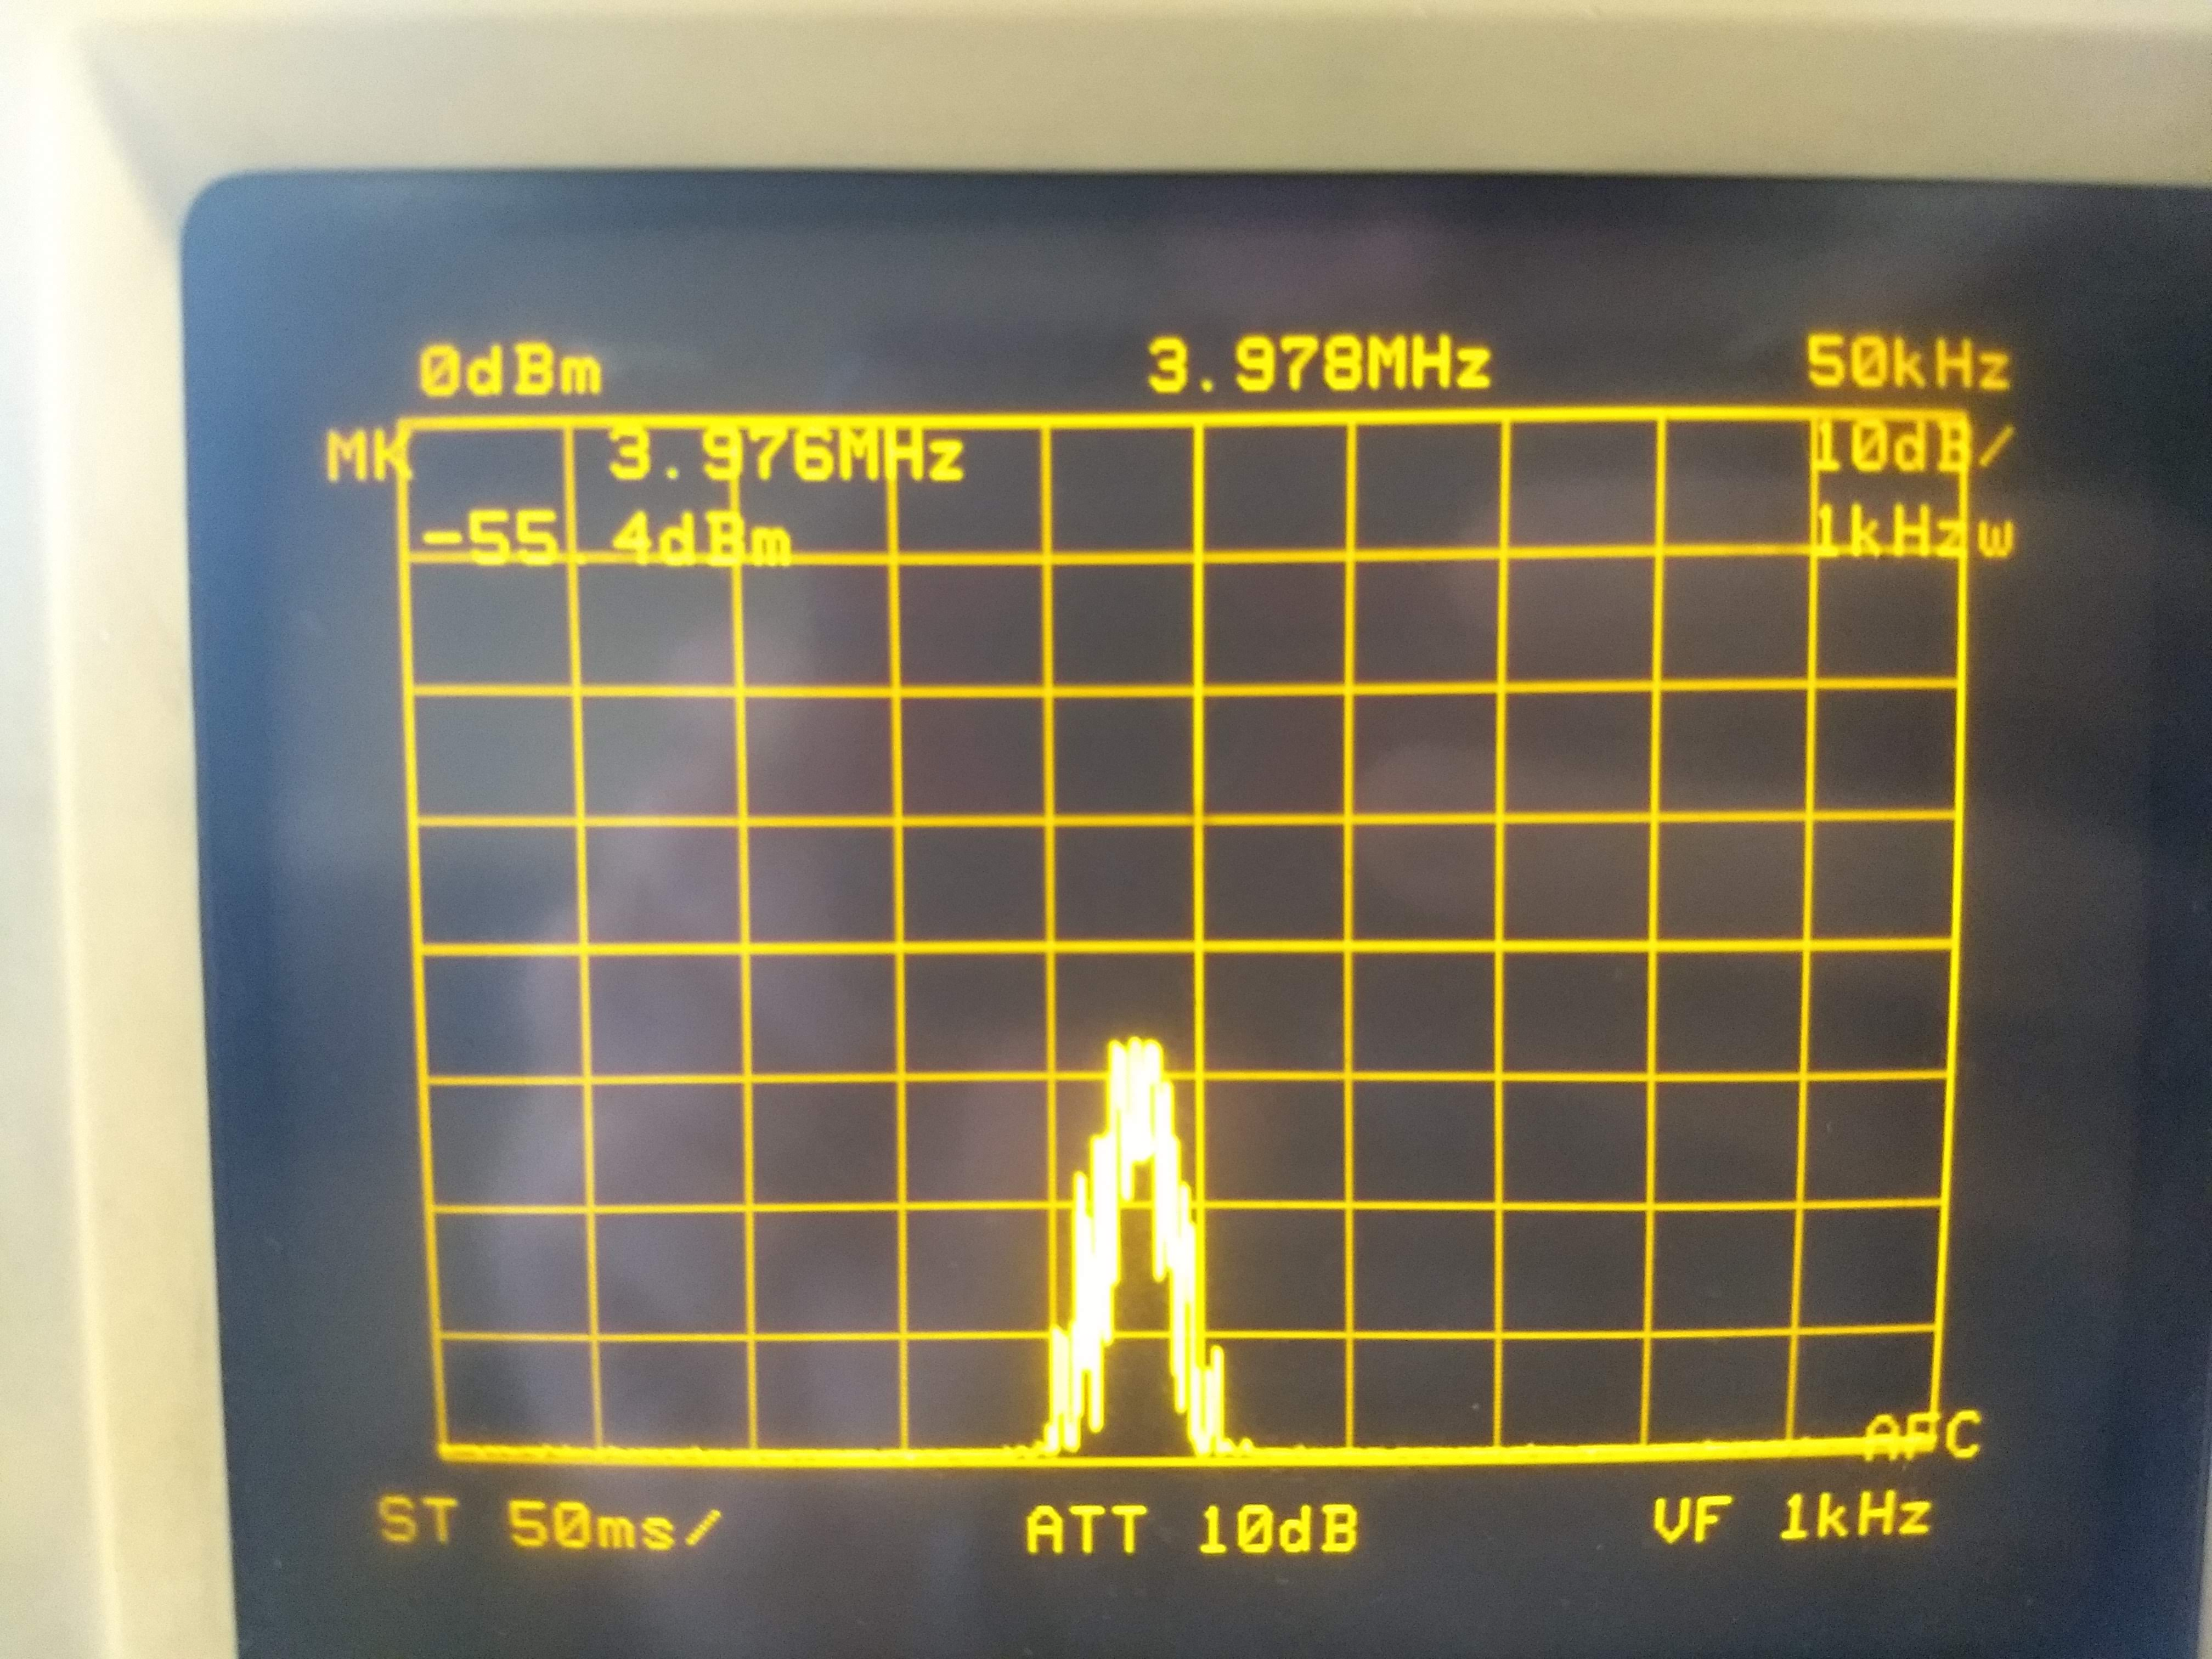
\includegraphics[width=\textwidth]{/ImagenesEjercicio1/gwP3.jpg}
    \caption{Tercer armónico para el generador GW}
    \label{fig:gw1}
  \end{minipage}
 \end{figure}

\subsection{Conclusiones}
Se puede concluir mediante las mediciones tomadas de los tres generadores de la distorsión armónica total que en este aspecto el generador de mayor calidad es el Agilent ya que no solo la distorsión armónica total calculada es menor a la de los otros tres tanto en la hoja de datos como efectivamente en la medición realizada. En este generador no eran apreciables los armónicos de orden mayor al primero debido al piso del ruido del analizador de espectros aún así con el atenuador en su mínima configuración. Luego, el generador cuya calidad se encuentra entre los otros dos es el Picotest, mientras que por un gran margen el generador GW es el de menor calidad.    
